\documentclass[polish,11pt,a4paper,twoside]{article}

\usepackage[utf8]{inputenc}
\usepackage[T1]{fontenc}
\usepackage[polish]{babel}
\usepackage[a4paper]{geometry}
\usepackage{listings}
\usepackage{graphicx}
\usepackage{amsthm}
\usepackage{color}
\usepackage{xcolor}
\usepackage{caption}
\usepackage{hyperref}
\usepackage{fancyhdr}
\usepackage{setspace}

\definecolor{light-gray}{gray}{0.95}

\lstset {
language=Java,
basicstyle=\footnotesize\ttfamily,
captionpos=t,
tabsize=2,
frame=lines,
keywordstyle=\color{blue},
commentstyle=\color{gray},
stringstyle=\color{red},
breaklines=true,
showstringspaces=false,
basicstyle=\footnotesize,
emph={label},
backgroundcolor=\color{light-gray}
}
\DeclareCaptionFont{white}{\color{white}}
\DeclareCaptionFormat{listing}{\colorbox{gray}{\parbox[c][0.25cm]{\textwidth}{#1#2#3}}}
\captionsetup[lstlisting]{format=listing,labelfont=white,textfont=white}

\parskip 10.0pt
\setlength{\parindent}{0cm}

\newenvironment{items}{
\begin{itemize}
  \setlength{\itemsep}{0pt}
  \setlength{\parskip}{0pt}
  \setlength{\parsep}{0pt}
  \setlength{\topsep}{0pt}
  \setlength{\partopsep}{0pt}
}{\end{itemize}}

 \renewcommand{\familydefault}{\sfdefault}

\begin{document}

\pagestyle{fancy}
\fancyhf{} % clear all header and footer fields
\fancyfoot[R]{\footnotesize \thepage}
\renewcommand{\headrulewidth}{0pt}
\renewcommand{\footrulewidth}{0pt}

\author{Olga Zachariasz,\\Aleksander Sobol,\\Bartłomiej Bułat,\\Bartłomiej Hyży,\\Julian Król,\\Łukasz Krzyżek,\\Maciej Gąsiorski,\\Tomasz Szczęśniak\\\\Informatyka Stosowana, IV rok\\WEAIiE, AGH}
\date{30.11.2011}
\title{Zarządzanie~projektami - komunikator programistów\\Dokumentacja techniczna}
\maketitle

\begin{spacing}{0.8}
\tableofcontents
\end{spacing}

\pagebreak

\thispagestyle{fancy}

\section{Analiza zadania}

\subsection{Cel projektu}

Celem projektu było przygotowanie narzędzia wspierającego zdalną pracę programistów nad kodem źródłowym aplikacji.

Zadaniem naszej grupy było przygotowanie specyficznego komunikatora internetowego - przeznaczonego dla programistów. Poza typową funkcjonalnością wymiany komunikatów tekstowych, jako wymaganie postawiona została możliwość wymiany plików źródłowych, nad którymi potem przeprowadzana miała być wspólna edycja - zaznaczanie fragmentów kodu i modyfikacja istniejącego kodu. Dodatkowo komunikacja miała przebiegać pomiędzy wieloma programistami na raz, na wzór rozmów konferencyjnych znanych ze standardowych komunikatorów.

Początkowo dodatkowymi wymaganiami była implementacja rozmów głosowych oraz możliwość połączeń peer-to-peer, ostatecznie jednak wynegcjowano porzucenie tych wymagań z uwagi na dużą złożoność implementacyjną.

Aplikacja miała działać na zasadzie klient-serwer oraz wspierać dwa systemy operacyjne: Microsoft Windows (XP, 7) oraz Linux (osobna paczka dla dystrybucji Debian).

\subsection{Komunikator - use case}
% use case komunikatora

\section{Wybór technologii}

% java, smack, xmpp, jabber, istniejace serwery, itp
Jako że pozostawiono wolną rękę co do wyboru technologii, w których wykonany miał być komunikator, zespół zdecydował się na wybór bibliotek i środowisk dobrze mu znanych:
\begin{itemize}
\item Język programowania - Java
\item IDE - NetBeans
\item Protokół komunikacji - XMPP\footnote{ang. Extensible Messaging and Presence Protocol - protokół bazujący na języku XML umożliwiający przesyłanie w czasie rzeczywistym wiadomości oraz statusu; protokół ma zastosowanie nie tylko w komunikatorach, ale również w innych systemach natychmiastowej wymiany informacji (źródło: Wikipedia)}
\item Biblioteka do komunikacji przez XMPP - Smack API\footnote{Strona domowa biblioteki: http://www.igniterealtime.org/projects/smack/}
\item Biblioteka GUI - Swing [?]
\end{itemize}

\section{Architektura komunikatora}

% klient nasz, serwer dowolny wlasciwie, rysunek
Na wybór protokołu XMPP do komunikacji pomiędzy programistami zdecydowano się głównie ze względu na jego otwartość, przystosowanie do rozszerzalności (np. o metadane informujące o edycji kodu) oraz użycie w wielu aplikacjach o podobnych możliwościach, służących do wspierania pracy grupowej zespołu programistów. Istotna okazała się również możliwość użycia istniejącej infrastruktury serwerów XMPP (dawniej Jabber), dzięki czemu wyeliminowana została konieczność implementacji programu serwera oraz dodatkowo zwiększona została niezawodność aplikacji, poprzez możliwość użycia do komunikacji dowolnego innego serwera w przypadku awarii aktualnie używanego.

Do komunikacji pomiędzy rozproszonymi klientami wybrany został serwer XMPP \emph{draugr.de}, gdyż umożliwia on niezbądne w implementowanej aplikacji rozmowy grupowe (ang. MUC - Multi User Chat) oraz rejestrację nowych kont użytkowników bezpośrednio w aplikacji, bez konieczności odwiedzania jego strony internetowej. Poglądowy schemat architektury systemu przedstawia rysunek \ref{fig:architektura}.

\begin{figure}[!htb]
  \begin{center}
    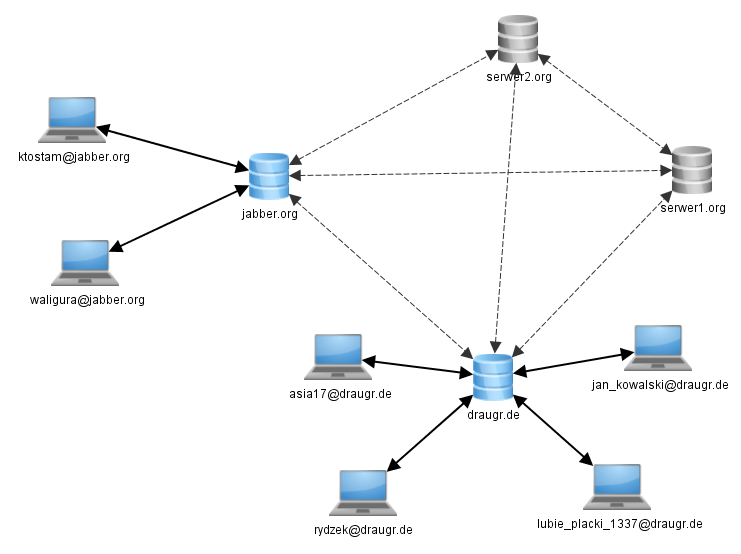
\includegraphics[width=1.0\textwidth]{img/architektura.png}
    \caption{Architektura klient-serwer komunikatora programistów} \label{fig:architektura} 
  \end{center}
\end{figure}

W aplikacji możliwe jest tworzenie nowych kont użytkowników tylko na serwerze \emph{draugr.de}, jednak możliwe jest użycie istniejącego konta z dowolnego innego serwera. Komunikacja użytkowników posiadających konta na tym samym serwerze odbywa się za pośrednictwem tego serwera. W przypadku gdy komunikacja następuje pomiędzy kontami na różnych serwerach, klient komunikatora wciąż wysyła swoje pakiety na swój serwer, zaś dopiero ten serwer przesyła go na serwer odbiorcy pakietu. Na rys. \ref{fig:architektura} liniami przerywanymi przedstawiono połączenia pomiędzy różnymi serwerami XMPP, nadzorującymi komunikację pomiędzy rozproszonymi po różnych serwerach klientami.

% \section{Podział na moduły}

% klient xmpp, gui, ...?
% jest sens?

\section{Klient XMPP}

% opis co to jest, ze opakowanie smack api, itp
Klient XMPP zaimplementowany został w postaci klasy \emph{XMPPClient}, której diagram przedstawiony jest na rys. \ref{fig:uml_class_client}. Klasa to korzysta bezpośrednio z biblioteki Smack API, stanowiącej niskopoziomową warstwę sieciową komunikatora. \emph{XMPPClient} implementuje wysokopoziome funkcjonalności pozwalające na wygodną abstrację pozostałej części aplikacji (graficznego interfejsu użytkownika) od szczegółów implementacyjnych komunikacji.
% schematy UML klas: XMPPClient, listener wiadomosci, itp.
\begin{figure}[!htb]
  \begin{center}
    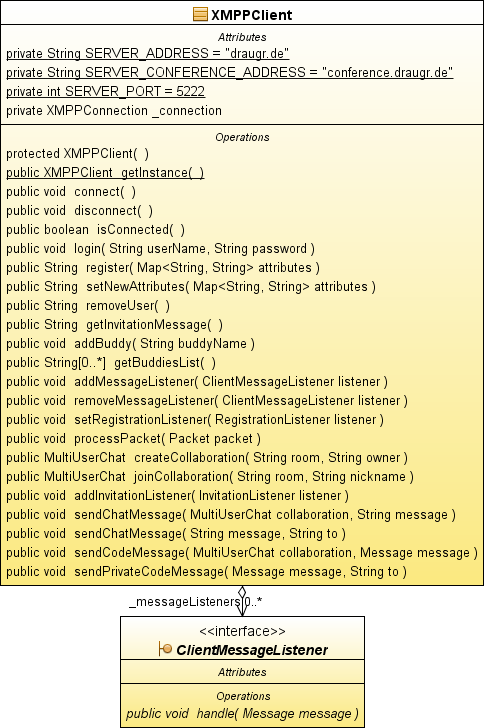
\includegraphics[width=0.9\textwidth]{img/uml_class_client.png}
    \caption{Diagram UML klas XMPPClient i ClientMessageListener} \label{fig:uml_class_client} 
  \end{center}
\end{figure}

Z punktu widzenia komunikatora najbardziej istotne są następujące funkcje:
\begin{items}
\item \emph{connect()}, \emph{disconnect()} - połączenie/rozłączanie się z serwerem
\item \emph{isConnected()} - sprawdzenie czy próba połączenia zakończyła się sukcesem
\item \emph{login()} - zalogowanie się na serwer XMPP jako istniejący użytkownik
\item \emph{register()} - zarejstrowanie nowego konta użytkownika na serwerze
\item \emph{addMessageListener()}, \emph{removeMessageListener()} - dodawanie i usuwanie nasłuchiwaczy wiadomości, patrz podrozdział \ref{sec:komunikacja}
\item \emph{processPacket()} - obsługa odbieranych pakietów, zawierających różnego rodzaju wiadomości
\item \emph{createCollaboration()}, \emph{joinCollaboration()} - tworzenie nowych i dołączanie do istniejących kolaboracji
\item \emph{sendChatMessage()}, \emph{sendCodeMessage()} - wysyłanie wiadomości tekstowych i wiadomości informujących o modyfikacji kodu źródłowego
\end{items}

\clearpage

\section{Komunikacja pomiędzy klientami}
\label{sec:komunikacja}

\subsection{Typy komunikatów}

% zwykła wiadomosc, wiadomosc gurpowa, metadane edycji kodu, itp
Celem realizacji przekazywania i interpretacji pakietów o różnych znaczeniach, zaimplementowana została rodzina klas wiadomości o różnych typach i różnych przeznaczeniach. Hierarchia tych klas przedstawiona jest na rys. \ref{fig:uml_class_message}.
\begin{figure}[!htb]
  \begin{center}
    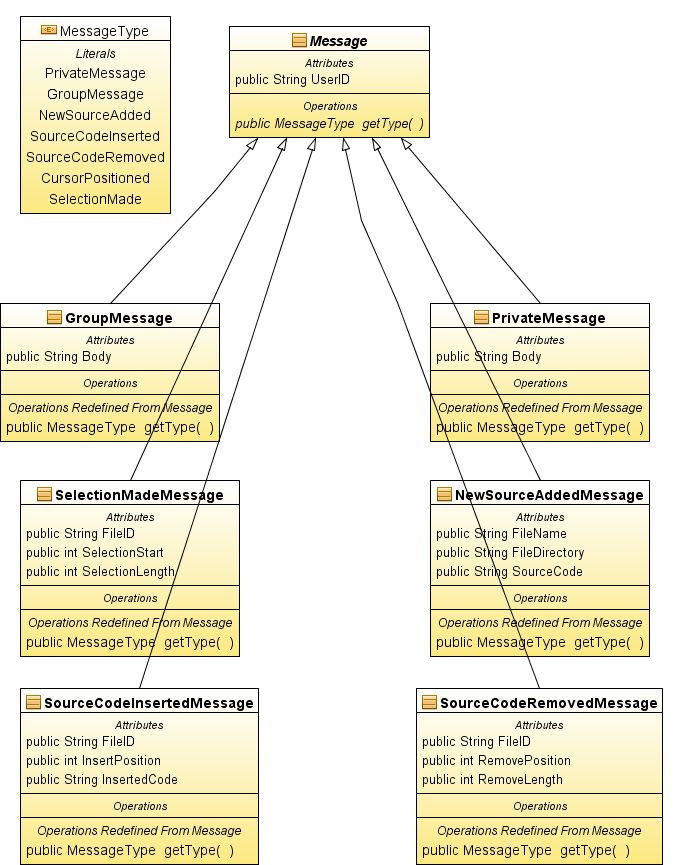
\includegraphics[width=0.9\textwidth]{img/uml_class_message.png}
    \caption{Diagram UML klas wiadomości} \label{fig:uml_class_message} 
  \end{center}
\end{figure}

Wszystkie klasy wiadomości dziedziczą po abstrakcyjnej bazie wiadomości - \emph{Message}. Zawiera ona jedynie pole \emph{UserID} z nazwą użytkownika-nadawcy wiadomości (np. \emph{alicja@draugr.de}) oraz abstrakcyjną metodę \emph{getType()}, która w klasach dziedziczących powinna być przeładowana celem zwracania swojego typu wiadomości jako jednej z wartości wyliczenia \emph{MessageType}. Dzięki temu możliwe jest odczytanie typu odebranej wiadomości i odpowiednia jej obsługa w zależności od tego typu (patrz przykład w \ref{sec:komPrzyklad}).

\emph{GroupMessage} i \emph{PrivateMessage} to wiadomości tekstowe, odpowiednio grupowe i prywatne. Zawierają pole Body z treścią wysłanej wiadomości.

Pozostałe wiadomości to klasy opisujące modyfikację plików źródłowych, nad którymi pracuje grupa programistów, w związku z czym zawierają dodatkowe metadane, np. \emph{FileID} - identyfikator pliku, do którego odnosi się wiadomość.

\emph{NewSourceAddedMessage} informuje o dodaniu do edycji nowego pliku źródłowego o nazwie \emph{FileName}, znajdującego się w katalogu \emph{FileDirectory} i mającego treść \emph{SourceCode}.

\emph{SelectionMadeMessage} informuje o zaznaczeniu przez programistę fragmentu kodu źródłowego z pliku \emph{FileID}, zaczynającym się na pozycji \emph{SelectionStart} i mającym \emph{SelectionLength} znaków.

\emph{SourceCodeInsertedMessage} informuje o dodaniu nowego fragmentu kodu do pliku o id. \emph{FileID}, zaczynającego się na pozycji \emph{InsertPosition} i składającego się ze znaków \emph{InsertedCode}.

\emph{SourceCodeRemovedMessage} informuje o usunięciu fragmentu kodu z pliku o id. \emph{FileID}, poczynając od pozycji \emph{InsertPosition}, o długości \emph{RemoveLength} znaków.

\emph{CursorPositioned} informuje o ustawieniu przez programistę kursora na pozycji \emph{CursorPosition} w pliku o id. \emph{FileID}.

\clearpage

\subsection{Przykład komunikacji}
\label{sec:komPrzyklad}

Rysunek \ref{fig:komunikacja} przedstawia przykładowy przepływ wiadomości pomiędzy użytkownikami komunikatora. W tym przypadku zaprezentowano przypadek, w którym jeden z programistów wprowadza zmiany do pliku źródłowego, nad którym pracuje grupa, w efekcie czego do reszty programistów (na rysynku zaprezentowano tylko jednego) trafia wiadomość pozwalającą na synchronizację stanu dokumentu.

% jeden klient wysyla cos do drugiego, na koncach podpiete listenery, ladny rysunek z ekranami, komunikatami, serwerami, itp
\begin{figure}[!htb]
  \begin{center}
    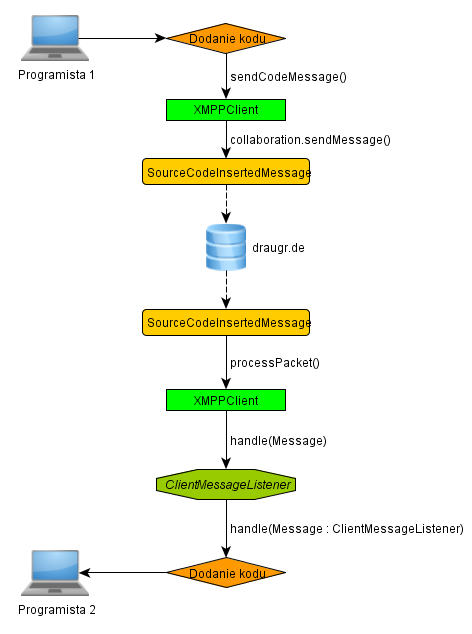
\includegraphics[width=0.9\textwidth]{img/komunikacja.png}
    \caption{Przykład przepływu wiadomości pomiędzy użytkownikami komunikatora} \label{fig:komunikacja} 
  \end{center}
\end{figure}

Użytkownik inicjuje przepływ pakietów poprzez dokonanie modyfikacji w kodzie lub wysłanie wiadomości tekstowej, co na rys. \ref{fig:komunikacja} symbolizuje ciemnopomarańczowy romb \emph{,,Dodanie kodu''}. Za interakcję z programistą i tłumaczenie jego działań na wiadomości oraz przesyłanie ich za pomocą \emph{XMPPClient} odpowiedzialny jest moduł GUI komunikatora.

Tak sporządzona wiadomość trafia na serwer XMPP, skąd jest rozsyłana do odpowiednich użytkowników - w przypadku wiadomości prywatnej do pojedynczego adresata, zaś w przypadku wiadomości grupowej do wszystkich członków kolaboracji.

Instancje klienta XMPP u adresatów otrzymują wiadomości, które następnie są przetwarzane przez klasy implementujące interfejs \emph{ClientMessageListener}. Pierwszym etapem takiego przetwarzania jest zrzutowanie otrzymanej wiadomości na odpowiedni typ, w zależności od wartości \emph{message.getType()}. Drugi, ostatni etap to obsłużenie konkretnej wiadomości w zależności od jej typu. Przykładowe przetwarzanie wiadomości przedstawia listing \ref{lst:listener}.

\begin{lstlisting}[label=lst:listener,caption=Przykład obsługi otrzymywanych wiadomości po stronie klienta XMPP]
public TestMsgListener implements ClientMessageListener {

  public void handle(Message message) {
    switch (message.getType()) {
      case NewSourceAdded:
        NewSourceAddedMessage msg = (NewSourceAddedMessage)message;
        // obsluz wiadomosc msg typu NewSourceAddedMessage
        break;
      case SourceCodeInserted:
        SourceCodeInsertedMessage msg = (SourceCodeInsertedMessage)message;
        // obsluz wiadomosc msg typu SourceCodeInserted
        break;
      // ... obsluga innych typow wiadomosci ...
    }
  }
}
\end{lstlisting}

\end{document}
